\documentclass[twoside]{book}

% Packages required by doxygen
\usepackage{fixltx2e}
\usepackage{calc}
\usepackage{doxygen}
\usepackage[export]{adjustbox} % also loads graphicx
\usepackage{graphicx}
\usepackage[utf8]{inputenc}
\usepackage{makeidx}
\usepackage{multicol}
\usepackage{multirow}
\PassOptionsToPackage{warn}{textcomp}
\usepackage{textcomp}
\usepackage[nointegrals]{wasysym}
\usepackage[table]{xcolor}

% Font selection
\usepackage[T1]{fontenc}
\usepackage[scaled=.90]{helvet}
\usepackage{courier}
\usepackage{amssymb}
\usepackage{sectsty}
\renewcommand{\familydefault}{\sfdefault}
\allsectionsfont{%
  \fontseries{bc}\selectfont%
  \color{darkgray}%
}
\renewcommand{\DoxyLabelFont}{%
  \fontseries{bc}\selectfont%
  \color{darkgray}%
}
\newcommand{\+}{\discretionary{\mbox{\scriptsize$\hookleftarrow$}}{}{}}

% Page & text layout
\usepackage{geometry}
\geometry{%
  a4paper,%
  top=2.5cm,%
  bottom=2.5cm,%
  left=2.5cm,%
  right=2.5cm%
}
\tolerance=750
\hfuzz=15pt
\hbadness=750
\setlength{\emergencystretch}{15pt}
\setlength{\parindent}{0cm}
\setlength{\parskip}{0.2cm}
\makeatletter
\renewcommand{\paragraph}{%
  \@startsection{paragraph}{4}{0ex}{-1.0ex}{1.0ex}{%
    \normalfont\normalsize\bfseries\SS@parafont%
  }%
}
\renewcommand{\subparagraph}{%
  \@startsection{subparagraph}{5}{0ex}{-1.0ex}{1.0ex}{%
    \normalfont\normalsize\bfseries\SS@subparafont%
  }%
}
\makeatother

% Headers & footers
\usepackage{fancyhdr}
\pagestyle{fancyplain}
\fancyhead[LE]{\fancyplain{}{\bfseries\thepage}}
\fancyhead[CE]{\fancyplain{}{}}
\fancyhead[RE]{\fancyplain{}{\bfseries\leftmark}}
\fancyhead[LO]{\fancyplain{}{\bfseries\rightmark}}
\fancyhead[CO]{\fancyplain{}{}}
\fancyhead[RO]{\fancyplain{}{\bfseries\thepage}}
\fancyfoot[LE]{\fancyplain{}{}}
\fancyfoot[CE]{\fancyplain{}{}}
\fancyfoot[RE]{\fancyplain{}{\bfseries\scriptsize Generated on Sun Nov 15 2015 14\+:25\+:31 for seng330ass2 by Doxygen }}
\fancyfoot[LO]{\fancyplain{}{\bfseries\scriptsize Generated on Sun Nov 15 2015 14\+:25\+:31 for seng330ass2 by Doxygen }}
\fancyfoot[CO]{\fancyplain{}{}}
\fancyfoot[RO]{\fancyplain{}{}}
\renewcommand{\footrulewidth}{0.4pt}
\renewcommand{\chaptermark}[1]{%
  \markboth{#1}{}%
}
\renewcommand{\sectionmark}[1]{%
  \markright{\thesection\ #1}%
}

% Indices & bibliography
\usepackage{natbib}
\usepackage[titles]{tocloft}
\setcounter{tocdepth}{3}
\setcounter{secnumdepth}{5}
\makeindex

% Hyperlinks (required, but should be loaded last)
\usepackage{ifpdf}
\ifpdf
  \usepackage[pdftex,pagebackref=true]{hyperref}
\else
  \usepackage[ps2pdf,pagebackref=true]{hyperref}
\fi
\hypersetup{%
  colorlinks=true,%
  linkcolor=blue,%
  citecolor=blue,%
  unicode%
}

% Custom commands
\newcommand{\clearemptydoublepage}{%
  \newpage{\pagestyle{empty}\cleardoublepage}%
}


%===== C O N T E N T S =====

\begin{document}

% Titlepage & ToC
\hypersetup{pageanchor=false,
             bookmarks=true,
             bookmarksnumbered=true,
             pdfencoding=unicode
            }
\pagenumbering{roman}
\begin{titlepage}
\vspace*{7cm}
\begin{center}%
{\Large seng330ass2 }\\
\vspace*{1cm}
{\large Generated by Doxygen 1.8.10}\\
\vspace*{0.5cm}
{\small Sun Nov 15 2015 14:25:31}\\
\end{center}
\end{titlepage}
\clearemptydoublepage
\tableofcontents
\clearemptydoublepage
\pagenumbering{arabic}
\hypersetup{pageanchor=true}

%--- Begin generated contents ---
\chapter{Hierarchical Index}
\section{Class Hierarchy}
This inheritance list is sorted roughly, but not completely, alphabetically\+:\begin{DoxyCompactList}
\item \contentsline{section}{Factory}{\pageref{class_factory}}{}
\item \contentsline{section}{Game\+Entity}{\pageref{class_game_entity}}{}
\begin{DoxyCompactList}
\item \contentsline{section}{Player}{\pageref{class_player}}{}
\item \contentsline{section}{Room}{\pageref{class_room}}{}
\end{DoxyCompactList}
\item Message\begin{DoxyCompactList}
\item \contentsline{section}{Person}{\pageref{class_person}}{}
\end{DoxyCompactList}
\item \contentsline{section}{Static\+Descriptor\+Initializer\+\_\+\+Game\+Entity\+\_\+2eproto}{\pageref{struct_static_descriptor_initializer___game_entity__2eproto}}{}
\end{DoxyCompactList}

\chapter{Class Index}
\section{Class List}
Here are the classes, structs, unions and interfaces with brief descriptions\+:\begin{DoxyCompactList}
\item\contentsline{section}{\hyperlink{class_factory}{Factory} }{\pageref{class_factory}}{}
\item\contentsline{section}{\hyperlink{class_game_entity}{Game\+Entity} }{\pageref{class_game_entity}}{}
\item\contentsline{section}{\hyperlink{class_person}{Person} }{\pageref{class_person}}{}
\item\contentsline{section}{\hyperlink{class_player}{Player} }{\pageref{class_player}}{}
\item\contentsline{section}{\hyperlink{class_room}{Room} }{\pageref{class_room}}{}
\item\contentsline{section}{\hyperlink{struct_static_descriptor_initializer___game_entity__2eproto}{Static\+Descriptor\+Initializer\+\_\+\+Game\+Entity\+\_\+2eproto} }{\pageref{struct_static_descriptor_initializer___game_entity__2eproto}}{}
\end{DoxyCompactList}

\chapter{Class Documentation}
\hypertarget{class_factory}{}\section{Factory Class Reference}
\label{class_factory}\index{Factory@{Factory}}
\subsection*{Static Public Member Functions}
\begin{DoxyCompactItemize}
\item 
static \hyperlink{class_game_entity}{Game\+Entity} $\ast$ \hyperlink{class_factory_a97476bf4211007c219698e840261eef1}{Make\+Game\+Entity} (int choice)
\end{DoxyCompactItemize}


\subsection{Member Function Documentation}
\hypertarget{class_factory_a97476bf4211007c219698e840261eef1}{}\index{Factory@{Factory}!Make\+Game\+Entity@{Make\+Game\+Entity}}
\index{Make\+Game\+Entity@{Make\+Game\+Entity}!Factory@{Factory}}
\subsubsection[{Make\+Game\+Entity(int choice)}]{\setlength{\rightskip}{0pt plus 5cm}{\bf Game\+Entity} $\ast$ Factory\+::\+Make\+Game\+Entity (
\begin{DoxyParamCaption}
\item[{int}]{choice}
\end{DoxyParamCaption}
)\hspace{0.3cm}{\ttfamily [static]}}\label{class_factory_a97476bf4211007c219698e840261eef1}
Clones a copy of object in prototypes array 

The documentation for this class was generated from the following files\+:\begin{DoxyCompactItemize}
\item 
Factory.\+h\item 
Factory.\+cpp\end{DoxyCompactItemize}

\hypertarget{class_game_entity}{}\section{Game\+Entity Class Reference}
\label{class_game_entity}\index{Game\+Entity@{Game\+Entity}}
Inheritance diagram for Game\+Entity\+:\begin{figure}[H]
\begin{center}
\leavevmode
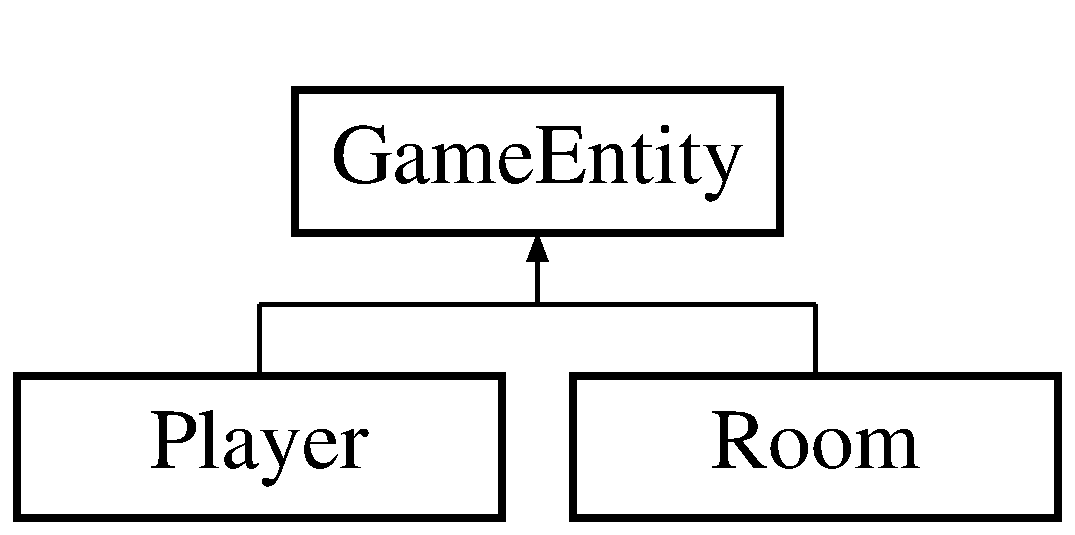
\includegraphics[height=3.000000cm]{class_game_entity}
\end{center}
\end{figure}
\subsection*{Public Member Functions}
\begin{DoxyCompactItemize}
\item 
\hyperlink{class_game_entity_a43e4841110c2de7e207d25cd31573616}{Game\+Entity} ()
\item 
\hypertarget{class_game_entity_ac534073fe3e7b25d95029c8af622a88e}{}{\bfseries Game\+Entity} (int id, std\+::string name)\label{class_game_entity_ac534073fe3e7b25d95029c8af622a88e}

\item 
\hypertarget{class_game_entity_a941b5c3c653f7526545bd81816e9531a}{}{\bfseries Game\+Entity} (int id, std\+::string name, std\+::string description)\label{class_game_entity_a941b5c3c653f7526545bd81816e9531a}

\item 
\hyperlink{class_game_entity_a241238b29b5e440107a5b295edf24f9c}{$\sim$\+Game\+Entity} ()
\item 
\hypertarget{class_game_entity_a0effae7533a6e242c71a5ccd2bb5a030}{}virtual \hyperlink{class_game_entity}{Game\+Entity} $\ast$ {\bfseries Clone} ()=0\label{class_game_entity_a0effae7533a6e242c71a5ccd2bb5a030}

\item 
void \hyperlink{class_game_entity_ac909a518389ee9bc92562b4166340766}{Print} ()
\item 
\hypertarget{class_game_entity_aab71ff714f47988b091fc40f2c30195a}{}void {\bfseries Print\+Name} ()\label{class_game_entity_aab71ff714f47988b091fc40f2c30195a}

\item 
int \hyperlink{class_game_entity_ad20b660a4f851e9636fdfd15f0d44df0}{Get\+Id} ()
\item 
\hypertarget{class_game_entity_ae45ee64de484dec1b16aea85171d9856}{}std\+::string {\bfseries Get\+Name} ()\label{class_game_entity_ae45ee64de484dec1b16aea85171d9856}

\item 
\hypertarget{class_game_entity_ac8da446a6c6990585b6581fe8537b7bf}{}std\+::string {\bfseries Get\+Description} ()\label{class_game_entity_ac8da446a6c6990585b6581fe8537b7bf}

\item 
void \hyperlink{class_game_entity_a5846ca63544cea04c672d51361e82537}{Set\+Id} (int id)
\item 
\hypertarget{class_game_entity_aa48a3a64bc80d6e199301b9d5bac4409}{}void {\bfseries Set\+Name} (std\+::string name)\label{class_game_entity_aa48a3a64bc80d6e199301b9d5bac4409}

\item 
\hypertarget{class_game_entity_a163f5785614921a65aab161491d8c47c}{}void {\bfseries Set\+Description} (std\+::string description)\label{class_game_entity_a163f5785614921a65aab161491d8c47c}

\item 
\hypertarget{class_game_entity_a8be507b6f8e3393e76d59b87b8dd8ec1}{}{\bfseries Game\+Entity} (const \hyperlink{class_game_entity}{Game\+Entity} \&from)\label{class_game_entity_a8be507b6f8e3393e76d59b87b8dd8ec1}

\item 
\hypertarget{class_game_entity_a9e1d3cf472239c42d097d4a417128ec9}{}\hyperlink{class_game_entity}{Game\+Entity} \& {\bfseries operator=} (const \hyperlink{class_game_entity}{Game\+Entity} \&from)\label{class_game_entity_a9e1d3cf472239c42d097d4a417128ec9}

\item 
\hypertarget{class_game_entity_a3d934514629d13e5eb05ba46db415616}{}const \+::google\+::protobuf\+::\+Unknown\+Field\+Set \& {\bfseries unknown\+\_\+fields} () const \label{class_game_entity_a3d934514629d13e5eb05ba46db415616}

\item 
\hypertarget{class_game_entity_a7ce79ef8a2b5fb69b8cf8fac2aa15a56}{}inline\+::google\+::protobuf\+::\+Unknown\+Field\+Set $\ast$ {\bfseries mutable\+\_\+unknown\+\_\+fields} ()\label{class_game_entity_a7ce79ef8a2b5fb69b8cf8fac2aa15a56}

\item 
\hypertarget{class_game_entity_aecf0195208966d0057722ccd68d054d5}{}void {\bfseries Swap} (\hyperlink{class_game_entity}{Game\+Entity} $\ast$other)\label{class_game_entity_aecf0195208966d0057722ccd68d054d5}

\item 
\hypertarget{class_game_entity_a5bfc2ef83277f013f48ccdbc91ed3939}{}\hyperlink{class_game_entity}{Game\+Entity} $\ast$ {\bfseries New} () const \label{class_game_entity_a5bfc2ef83277f013f48ccdbc91ed3939}

\item 
\hypertarget{class_game_entity_ad564106c4c0219fdaae20cc89a1f9eab}{}void {\bfseries Copy\+From} (const \+::google\+::protobuf\+::\+Message \&from)\label{class_game_entity_ad564106c4c0219fdaae20cc89a1f9eab}

\item 
\hypertarget{class_game_entity_ad962a6322eab070b8237fdf225601483}{}void {\bfseries Merge\+From} (const \+::google\+::protobuf\+::\+Message \&from)\label{class_game_entity_ad962a6322eab070b8237fdf225601483}

\item 
\hypertarget{class_game_entity_ad2e29c89bb229fe7947d5ee8a61001fb}{}void {\bfseries Copy\+From} (const \hyperlink{class_game_entity}{Game\+Entity} \&from)\label{class_game_entity_ad2e29c89bb229fe7947d5ee8a61001fb}

\item 
\hypertarget{class_game_entity_aee3cabc70886a412c84f7046d8f0a28e}{}void {\bfseries Merge\+From} (const \hyperlink{class_game_entity}{Game\+Entity} \&from)\label{class_game_entity_aee3cabc70886a412c84f7046d8f0a28e}

\item 
\hypertarget{class_game_entity_afd155897472b7f1eb218556ce98d6a9b}{}void {\bfseries Clear} ()\label{class_game_entity_afd155897472b7f1eb218556ce98d6a9b}

\item 
\hypertarget{class_game_entity_afa6583197e095273509d30ad6592f56b}{}bool {\bfseries Is\+Initialized} () const \label{class_game_entity_afa6583197e095273509d30ad6592f56b}

\item 
\hypertarget{class_game_entity_a1427623c35bf6e2f89bb300e4d339141}{}int {\bfseries Byte\+Size} () const \label{class_game_entity_a1427623c35bf6e2f89bb300e4d339141}

\item 
\hypertarget{class_game_entity_a78b3ff51c8c5f3162abc072d080baabf}{}bool {\bfseries Merge\+Partial\+From\+Coded\+Stream} (\+::google\+::protobuf\+::io\+::\+Coded\+Input\+Stream $\ast$input)\label{class_game_entity_a78b3ff51c8c5f3162abc072d080baabf}

\item 
\hypertarget{class_game_entity_a704014c07ab7cb693c2b4590ca645b33}{}void {\bfseries Serialize\+With\+Cached\+Sizes} (\+::google\+::protobuf\+::io\+::\+Coded\+Output\+Stream $\ast$output) const \label{class_game_entity_a704014c07ab7cb693c2b4590ca645b33}

\item 
\hypertarget{class_game_entity_a9c3c2e602eb8393c6df678857757e035}{}\+::google\+::protobuf\+::uint8 $\ast$ {\bfseries Serialize\+With\+Cached\+Sizes\+To\+Array} (\+::google\+::protobuf\+::uint8 $\ast$output) const \label{class_game_entity_a9c3c2e602eb8393c6df678857757e035}

\item 
\hypertarget{class_game_entity_a48549bd37abe3683e99dd11146ef002f}{}int {\bfseries Get\+Cached\+Size} () const \label{class_game_entity_a48549bd37abe3683e99dd11146ef002f}

\item 
\hypertarget{class_game_entity_aac721e84e4bde7e73558dc1b705b3368}{}\+::google\+::protobuf\+::\+Metadata {\bfseries Get\+Metadata} () const \label{class_game_entity_aac721e84e4bde7e73558dc1b705b3368}

\item 
\hypertarget{class_game_entity_ae5a31e6e2821400231140a09a6a6fd67}{}bool {\bfseries has\+\_\+id} () const \label{class_game_entity_ae5a31e6e2821400231140a09a6a6fd67}

\item 
\hypertarget{class_game_entity_adabd08d52e2c6389aff70a80461f45b3}{}void {\bfseries clear\+\_\+id} ()\label{class_game_entity_adabd08d52e2c6389aff70a80461f45b3}

\item 
\hypertarget{class_game_entity_af05a09cc0df4c9e742b3a4c3d6c698ca}{}inline\+::google\+::protobuf\+::int32 {\bfseries id} () const \label{class_game_entity_af05a09cc0df4c9e742b3a4c3d6c698ca}

\item 
\hypertarget{class_game_entity_a2ebfb94e8e4796971d865d2422df496b}{}void {\bfseries set\+\_\+id} (\+::google\+::protobuf\+::int32 value)\label{class_game_entity_a2ebfb94e8e4796971d865d2422df496b}

\item 
\hypertarget{class_game_entity_a88030133de49f7fe670330e3cc929b6b}{}bool {\bfseries has\+\_\+name} () const \label{class_game_entity_a88030133de49f7fe670330e3cc929b6b}

\item 
\hypertarget{class_game_entity_af2da515bc6f89f976618f066e7ce2d0c}{}void {\bfseries clear\+\_\+name} ()\label{class_game_entity_af2da515bc6f89f976618f066e7ce2d0c}

\item 
\hypertarget{class_game_entity_a40520ca73e5569e7914053bb93ec7092}{}const \+::std\+::string \& {\bfseries name} () const \label{class_game_entity_a40520ca73e5569e7914053bb93ec7092}

\item 
\hypertarget{class_game_entity_a7ad33d3d3201374885cd4460f15662f6}{}void {\bfseries set\+\_\+name} (const \+::std\+::string \&value)\label{class_game_entity_a7ad33d3d3201374885cd4460f15662f6}

\item 
\hypertarget{class_game_entity_a6a4ff6c04ca52c8d94090f7c556673d5}{}void {\bfseries set\+\_\+name} (const char $\ast$value)\label{class_game_entity_a6a4ff6c04ca52c8d94090f7c556673d5}

\item 
\hypertarget{class_game_entity_a7004ef266061469a6b39052baf579cf9}{}void {\bfseries set\+\_\+name} (const char $\ast$value, size\+\_\+t size)\label{class_game_entity_a7004ef266061469a6b39052baf579cf9}

\item 
\hypertarget{class_game_entity_a81a39f375d3e5914d3339d45d518233b}{}inline\+::std\+::string $\ast$ {\bfseries mutable\+\_\+name} ()\label{class_game_entity_a81a39f375d3e5914d3339d45d518233b}

\item 
\hypertarget{class_game_entity_a22cff7dee6991f873fe096ba82230988}{}inline\+::std\+::string $\ast$ {\bfseries release\+\_\+name} ()\label{class_game_entity_a22cff7dee6991f873fe096ba82230988}

\item 
\hypertarget{class_game_entity_a92c6ebce60eff2803ff387af4b867da0}{}void {\bfseries set\+\_\+allocated\+\_\+name} (\+::std\+::string $\ast$name)\label{class_game_entity_a92c6ebce60eff2803ff387af4b867da0}

\item 
\hypertarget{class_game_entity_a95649eb24f47bac1152da548d34fb742}{}bool {\bfseries has\+\_\+description} () const \label{class_game_entity_a95649eb24f47bac1152da548d34fb742}

\item 
\hypertarget{class_game_entity_a72fb20413ba6dde033f5c2179c053f99}{}void {\bfseries clear\+\_\+description} ()\label{class_game_entity_a72fb20413ba6dde033f5c2179c053f99}

\item 
\hypertarget{class_game_entity_a3441f1430479ddb262dd3535112ab901}{}const \+::std\+::string \& {\bfseries description} () const \label{class_game_entity_a3441f1430479ddb262dd3535112ab901}

\item 
\hypertarget{class_game_entity_ad836eb0089916b4959a73e015d154408}{}void {\bfseries set\+\_\+description} (const \+::std\+::string \&value)\label{class_game_entity_ad836eb0089916b4959a73e015d154408}

\item 
\hypertarget{class_game_entity_a381d51b25532bdec6f852cc4a10221c0}{}void {\bfseries set\+\_\+description} (const char $\ast$value)\label{class_game_entity_a381d51b25532bdec6f852cc4a10221c0}

\item 
\hypertarget{class_game_entity_a2e744ca8dbddbfa72f06b0681fd3ad6f}{}void {\bfseries set\+\_\+description} (const char $\ast$value, size\+\_\+t size)\label{class_game_entity_a2e744ca8dbddbfa72f06b0681fd3ad6f}

\item 
\hypertarget{class_game_entity_ad3928cb09cd351152f0d61bde3b177d8}{}inline\+::std\+::string $\ast$ {\bfseries mutable\+\_\+description} ()\label{class_game_entity_ad3928cb09cd351152f0d61bde3b177d8}

\item 
\hypertarget{class_game_entity_ad6ddcad96329b910af7708d7fe195fd2}{}inline\+::std\+::string $\ast$ {\bfseries release\+\_\+description} ()\label{class_game_entity_ad6ddcad96329b910af7708d7fe195fd2}

\item 
\hypertarget{class_game_entity_a0247fb1afaf6f4c78e556613ca878206}{}void {\bfseries set\+\_\+allocated\+\_\+description} (\+::std\+::string $\ast$description)\label{class_game_entity_a0247fb1afaf6f4c78e556613ca878206}

\end{DoxyCompactItemize}
\subsection*{Static Public Member Functions}
\begin{DoxyCompactItemize}
\item 
\hypertarget{class_game_entity_a96a51564257590278f571b71836b7b0f}{}static const \+::google\+::protobuf\+::\+Descriptor $\ast$ {\bfseries descriptor} ()\label{class_game_entity_a96a51564257590278f571b71836b7b0f}

\item 
\hypertarget{class_game_entity_ab5cdaf2b5b95f303770216e9c84ea5b5}{}static const \hyperlink{class_game_entity}{Game\+Entity} \& {\bfseries default\+\_\+instance} ()\label{class_game_entity_ab5cdaf2b5b95f303770216e9c84ea5b5}

\end{DoxyCompactItemize}
\subsection*{Static Public Attributes}
\begin{DoxyCompactItemize}
\item 
\hypertarget{class_game_entity_aa83493bf7e483e028cb07bffe1dfdd27}{}static const int {\bfseries k\+Id\+Field\+Number} = 1\label{class_game_entity_aa83493bf7e483e028cb07bffe1dfdd27}

\item 
\hypertarget{class_game_entity_a965f608a057f6571cb60ac889572608a}{}static const int {\bfseries k\+Name\+Field\+Number} = 2\label{class_game_entity_a965f608a057f6571cb60ac889572608a}

\item 
\hypertarget{class_game_entity_adecaf52bd2eb80bfa8564744a5e4252b}{}static const int {\bfseries k\+Description\+Field\+Number} = 3\label{class_game_entity_adecaf52bd2eb80bfa8564744a5e4252b}

\end{DoxyCompactItemize}
\subsection*{Friends}
\begin{DoxyCompactItemize}
\item 
\hypertarget{class_game_entity_a4dde39854f794a3b19e2b7b55c4b6b06}{}void {\bfseries protobuf\+\_\+\+Add\+Desc\+\_\+\+Game\+Entity\+\_\+2eproto} ()\label{class_game_entity_a4dde39854f794a3b19e2b7b55c4b6b06}

\item 
\hypertarget{class_game_entity_af238f5cf048f1dd08b479e04ecbe1573}{}void {\bfseries protobuf\+\_\+\+Assign\+Desc\+\_\+\+Game\+Entity\+\_\+2eproto} ()\label{class_game_entity_af238f5cf048f1dd08b479e04ecbe1573}

\item 
\hypertarget{class_game_entity_af5ab48289049b21ebe96df027c0dddb0}{}void {\bfseries protobuf\+\_\+\+Shutdown\+File\+\_\+\+Game\+Entity\+\_\+2eproto} ()\label{class_game_entity_af5ab48289049b21ebe96df027c0dddb0}

\end{DoxyCompactItemize}


\subsection{Constructor \& Destructor Documentation}
\hypertarget{class_game_entity_a43e4841110c2de7e207d25cd31573616}{}\index{Game\+Entity@{Game\+Entity}!Game\+Entity@{Game\+Entity}}
\index{Game\+Entity@{Game\+Entity}!Game\+Entity@{Game\+Entity}}
\subsubsection[{Game\+Entity()}]{\setlength{\rightskip}{0pt plus 5cm}Game\+Entity\+::\+Game\+Entity (
\begin{DoxyParamCaption}
{}
\end{DoxyParamCaption}
)}\label{class_game_entity_a43e4841110c2de7e207d25cd31573616}
constructors, one for each possibility of initial variables \hypertarget{class_game_entity_a241238b29b5e440107a5b295edf24f9c}{}\index{Game\+Entity@{Game\+Entity}!````~Game\+Entity@{$\sim$\+Game\+Entity}}
\index{````~Game\+Entity@{$\sim$\+Game\+Entity}!Game\+Entity@{Game\+Entity}}
\subsubsection[{$\sim$\+Game\+Entity()}]{\setlength{\rightskip}{0pt plus 5cm}Game\+Entity\+::$\sim$\+Game\+Entity (
\begin{DoxyParamCaption}
{}
\end{DoxyParamCaption}
)}\label{class_game_entity_a241238b29b5e440107a5b295edf24f9c}
destructor 

\subsection{Member Function Documentation}
\hypertarget{class_game_entity_ad20b660a4f851e9636fdfd15f0d44df0}{}\index{Game\+Entity@{Game\+Entity}!Get\+Id@{Get\+Id}}
\index{Get\+Id@{Get\+Id}!Game\+Entity@{Game\+Entity}}
\subsubsection[{Get\+Id()}]{\setlength{\rightskip}{0pt plus 5cm}int Game\+Entity\+::\+Get\+Id (
\begin{DoxyParamCaption}
{}
\end{DoxyParamCaption}
)}\label{class_game_entity_ad20b660a4f851e9636fdfd15f0d44df0}
getters \hypertarget{class_game_entity_ac909a518389ee9bc92562b4166340766}{}\index{Game\+Entity@{Game\+Entity}!Print@{Print}}
\index{Print@{Print}!Game\+Entity@{Game\+Entity}}
\subsubsection[{Print()}]{\setlength{\rightskip}{0pt plus 5cm}void Game\+Entity\+::\+Print (
\begin{DoxyParamCaption}
{}
\end{DoxyParamCaption}
)}\label{class_game_entity_ac909a518389ee9bc92562b4166340766}
print out information \hypertarget{class_game_entity_a5846ca63544cea04c672d51361e82537}{}\index{Game\+Entity@{Game\+Entity}!Set\+Id@{Set\+Id}}
\index{Set\+Id@{Set\+Id}!Game\+Entity@{Game\+Entity}}
\subsubsection[{Set\+Id(int id)}]{\setlength{\rightskip}{0pt plus 5cm}void Game\+Entity\+::\+Set\+Id (
\begin{DoxyParamCaption}
\item[{int}]{id}
\end{DoxyParamCaption}
)}\label{class_game_entity_a5846ca63544cea04c672d51361e82537}
setters 

The documentation for this class was generated from the following files\+:\begin{DoxyCompactItemize}
\item 
Game\+Entity.\+h\item 
Game\+Entity.\+pb.\+h\item 
Game\+Entity.\+cpp\item 
Game\+Entity.\+pb.\+cc\end{DoxyCompactItemize}

\hypertarget{class_player}{}\section{Player Class Reference}
\label{class_player}\index{Player@{Player}}
Inheritance diagram for Player\+:\begin{figure}[H]
\begin{center}
\leavevmode
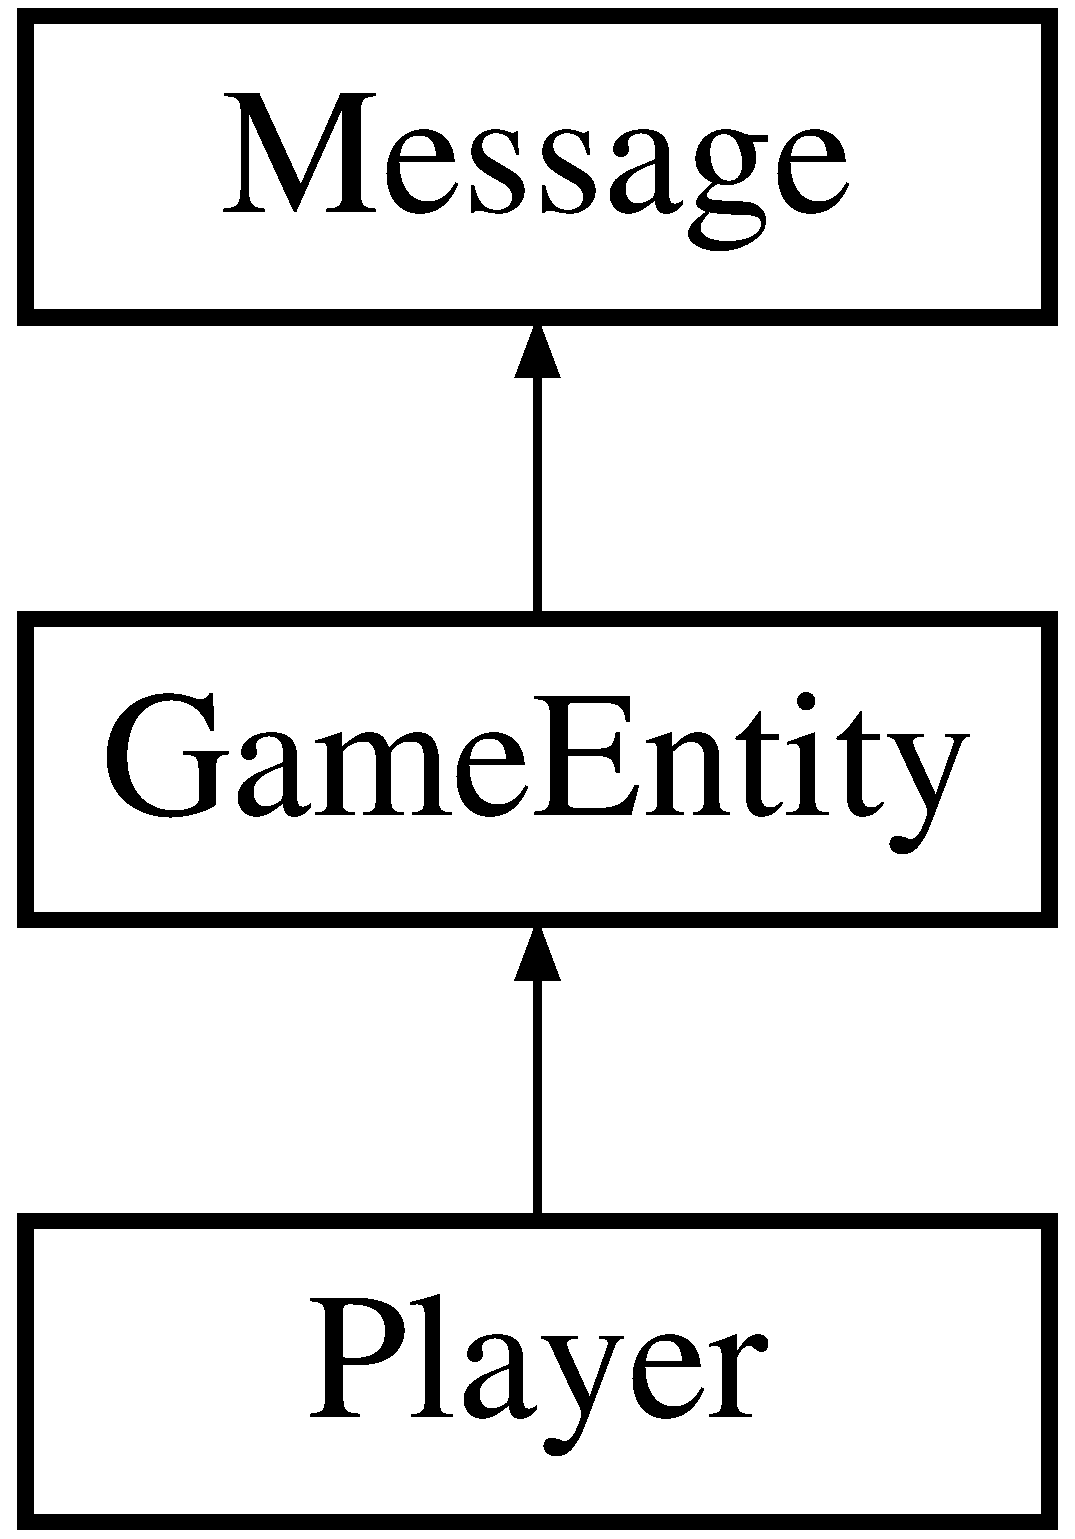
\includegraphics[height=3.000000cm]{class_player}
\end{center}
\end{figure}
\subsection*{Public Member Functions}
\begin{DoxyCompactItemize}
\item 
\hyperlink{class_player_affe0cc3cb714f6deb4e62f0c0d3f1fd8}{Player} ()
\item 
\hypertarget{class_player_a52b1205956ebebdf8fb8ed36cb96bb38}{}{\bfseries Player} (int id, std\+::string name)\label{class_player_a52b1205956ebebdf8fb8ed36cb96bb38}

\item 
\hypertarget{class_player_aece2ef9f10fff6f075e6690c3151ca7e}{}{\bfseries Player} (int id, std\+::string name, std\+::string description)\label{class_player_aece2ef9f10fff6f075e6690c3151ca7e}

\item 
\hyperlink{class_player_a749d2c00e1fe0f5c2746f7505a58c062}{$\sim$\+Player} ()
\item 
\hyperlink{class_player}{Player} $\ast$ \hyperlink{class_player_af5b2efe38828c633dc18228ce427177b}{Clone} ()
\end{DoxyCompactItemize}
\subsection*{Additional Inherited Members}


\subsection{Constructor \& Destructor Documentation}
\hypertarget{class_player_affe0cc3cb714f6deb4e62f0c0d3f1fd8}{}\index{Player@{Player}!Player@{Player}}
\index{Player@{Player}!Player@{Player}}
\subsubsection[{Player()}]{\setlength{\rightskip}{0pt plus 5cm}Player\+::\+Player (
\begin{DoxyParamCaption}
{}
\end{DoxyParamCaption}
)}\label{class_player_affe0cc3cb714f6deb4e62f0c0d3f1fd8}
\hyperlink{class_player}{Player} Constructors, use \hyperlink{class_game_entity}{Game\+Entity} constructor \hypertarget{class_player_a749d2c00e1fe0f5c2746f7505a58c062}{}\index{Player@{Player}!````~Player@{$\sim$\+Player}}
\index{````~Player@{$\sim$\+Player}!Player@{Player}}
\subsubsection[{$\sim$\+Player()}]{\setlength{\rightskip}{0pt plus 5cm}Player\+::$\sim$\+Player (
\begin{DoxyParamCaption}
{}
\end{DoxyParamCaption}
)}\label{class_player_a749d2c00e1fe0f5c2746f7505a58c062}
\hyperlink{class_player}{Player} Deconstructor 

\subsection{Member Function Documentation}
\hypertarget{class_player_af5b2efe38828c633dc18228ce427177b}{}\index{Player@{Player}!Clone@{Clone}}
\index{Clone@{Clone}!Player@{Player}}
\subsubsection[{Clone()}]{\setlength{\rightskip}{0pt plus 5cm}{\bf Player} $\ast$ Player\+::\+Clone (
\begin{DoxyParamCaption}
{}
\end{DoxyParamCaption}
)\hspace{0.3cm}{\ttfamily [virtual]}}\label{class_player_af5b2efe38828c633dc18228ce427177b}
Clones a player, returns empty object 

Implements \hyperlink{class_game_entity}{Game\+Entity}.



The documentation for this class was generated from the following files\+:\begin{DoxyCompactItemize}
\item 
Player.\+h\item 
Player.\+cpp\end{DoxyCompactItemize}

\hypertarget{class_room}{}\section{Room Class Reference}
\label{class_room}\index{Room@{Room}}
Inheritance diagram for Room\+:\begin{figure}[H]
\begin{center}
\leavevmode
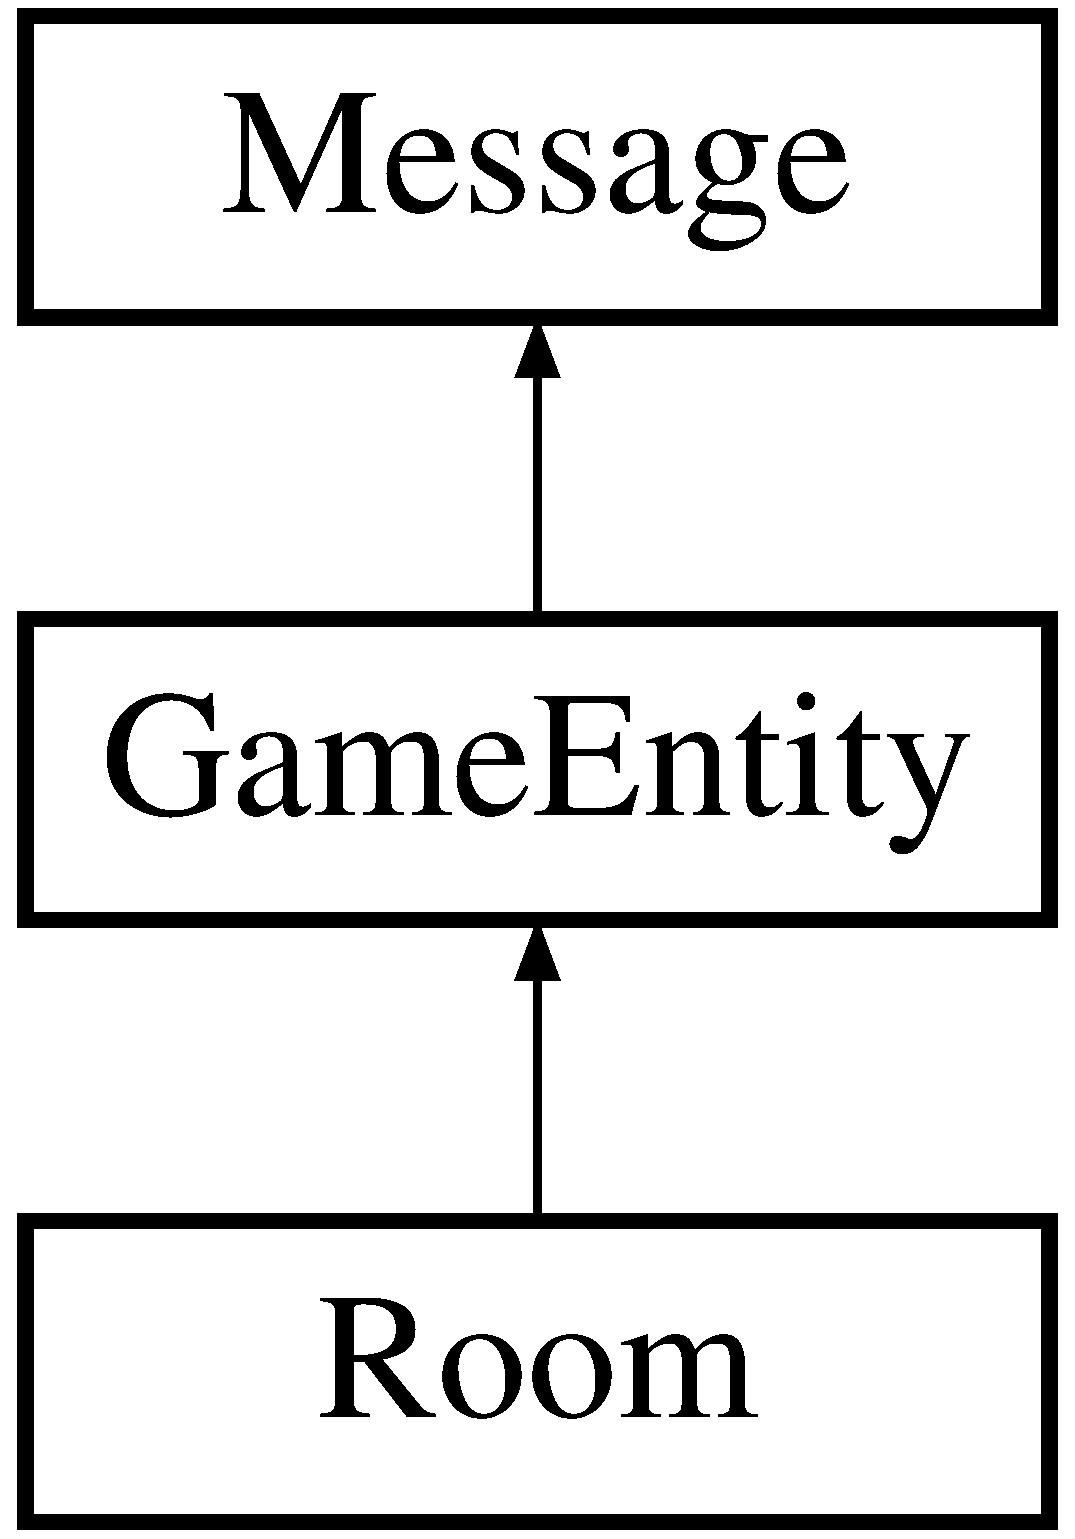
\includegraphics[height=2.000000cm]{class_room}
\end{center}
\end{figure}
\subsection*{Public Member Functions}
\begin{DoxyCompactItemize}
\item 
\hypertarget{class_room_a7e42f2ddca1d0fde48feabbf4eb06a80}{}{\bfseries Room} (int id, std\+::string description)\label{class_room_a7e42f2ddca1d0fde48feabbf4eb06a80}

\item 
\hypertarget{class_room_a2286569deae9af3cafc5716ce72dcbf1}{}{\bfseries Room} (int id, std\+::string name, std\+::string description)\label{class_room_a2286569deae9af3cafc5716ce72dcbf1}

\item 
\hypertarget{class_room_a15e3463eb05ec8de060d67fb11f6688d}{}\hyperlink{class_room}{Room} $\ast$ {\bfseries Clone} ()\label{class_room_a15e3463eb05ec8de060d67fb11f6688d}

\end{DoxyCompactItemize}


The documentation for this class was generated from the following files\+:\begin{DoxyCompactItemize}
\item 
Room.\+h\item 
Room.\+cpp\end{DoxyCompactItemize}

\hypertarget{struct_static_descriptor_initializer___game_entity__2eproto}{}\section{Static\+Descriptor\+Initializer\+\_\+\+Game\+Entity\+\_\+2eproto Struct Reference}
\label{struct_static_descriptor_initializer___game_entity__2eproto}\index{Static\+Descriptor\+Initializer\+\_\+\+Game\+Entity\+\_\+2eproto@{Static\+Descriptor\+Initializer\+\_\+\+Game\+Entity\+\_\+2eproto}}


The documentation for this struct was generated from the following file\+:\begin{DoxyCompactItemize}
\item 
Game\+Entity.\+pb.\+cc\end{DoxyCompactItemize}

%--- End generated contents ---

% Index
\backmatter
\newpage
\phantomsection
\clearemptydoublepage
\addcontentsline{toc}{chapter}{Index}
\printindex

\end{document}
